\chapter{Intro}
\section{The Internet}
\begin{itemize}[nosep]
    \item Collection of nodes, wired and wireless technology connecting these nodes, applications and services
    \item Types of nodes
          \begin{itemize}[nosep]
              \item Desktops and Laptop
              \item Servers
              \item TV/Refrigerator
              \item Cellphones
          \end{itemize}
    \item Goal: Connect all the nodes to each other
    \item Solutions
          \begin{itemize}[nosep]
              \item $\binom{n}{2} = \bigO{n^2}$ cables
              \item Sharing the links
                    \begin{itemize}[nosep]
                        \item Circuit Switching
                        \item Packet Switching
                    \end{itemize}
          \end{itemize}
    \item Packet
          \begin{itemize}[nosep]
              \item Collection of bits to transfer across a network
              \item Think: envelope and its contents
          \end{itemize}
    \item Circuit
          \begin{itemize}[nosep]
              \item Pre-allocated path/resource
          \end{itemize}
\end{itemize}
\section{Packet vs. Circuit Switching}
\begin{figure}[H]
    \begin{tikzpicture}[every node/.style={white, draw=blue, circle, minimum size=1cm, fill=blue}]
        \node[top color=blue!30!white, bottom color=blue!60!white] (a) {$A$};
        \node[top color=blue!30!white, bottom color=blue!60!white,below=of a] (b) {$B$};
        \node[top color=blue!30!white, bottom color=blue!60!white,below=of b] (c) {$C$};

        \node[top color=blue!30!white, bottom color=blue!60!white,right=2cm of b, minimum height=1.25cm, minimum width=2cm, rectangle, rounded corners] (r) {};

        \node[top color=blue!30!white, bottom color=blue!60!white,right=2cm of r] (d) {$D$};
        \draw[blue!90!white, ->] (a) -- ([yshift=0.2cm,xshift=0.3cm]r.west);
        \draw[blue!90!white, ->] (b) -- ([xshift=0.3cm]r.west);
        \draw[blue!90!white, ->] (c) -- ([yshift=-0.2cm,xshift=0.3cm]r.west);
        \draw[blue!90!white, ->, thick] (r.east) -- (d);
        \path ([yshift=-1cm]r.south west) -- ([yshift=-1cm]r.south east) node[style={align=center,black,draw=none,fill=none},pos=0.5] {Wireless AP\\Switch\\Router};
    \end{tikzpicture}
\end{figure}
\subsection{Circuit Switching}
\begin{itemize}[nosep]
    \item Setup the connection or resource
          \begin{itemize}[nosep]
              \item Schedule (e.g., TDMA)
              \item State in the network
          \end{itemize}
\end{itemize}
\begin{multicols}{2}
    \begin{figure}[H]
        \begin{tikzpicture}[every node/.style={rectangle, draw=blue!60!white, minimum size=1cm}]
            \node (a) {$A$};
            \node[below=of a] (b) {$B$};

            \node[below right=-0.4cm and 1cm of a, minimum width=3cm, minimum height=2cm] (s) {Switch};

            \node[above right=-0.4cm and 1cm of s] (c) {$C$};
            \node[below right=-0.4cm and 1cm of s] (d) {$D$};

            \draw[blue!60!white] (a) -- (s);
            \draw[blue!60!white] (b) -- (s);
            \draw[blue!60!white] (c) -- (s);
            \draw[blue!60!white] (d) -- (s);
        \end{tikzpicture}
    \end{figure}

    \begin{table}[H]
        \begin{tabular}{l l}
            Time                      & Circuit \\\toprule
            $T$, $3T$, $5T$, $\dots$  & $A - D$ \\
            $2T$, $4T$, $6T$, $\dots$ & $B - C$
        \end{tabular}
    \end{table}
\end{multicols}
\begin{itemize}[nosep]
    \item Natural for predictable data races
    \item Can guarantee certain level of services
    \item Can be inefficient for many applications
\end{itemize}
\subsection{Some Circuit Switching Techniques}
\begin{itemize}[nosep]
    \item Time
          \begin{itemize}[nosep]
              \item Reserve to use the link at a given schedule
              \item Read: \url{https://en.wikipedia.org/wiki/Time-division_multiplexing}
          \end{itemize}
    \item Frequency
          \begin{itemize}[nosep]
              \item Reserve to use certain frequencies (channel)
              \item Read: \url{https://en.wikipedia.org/wiki/Frequency-division_multiplexing}
          \end{itemize}
\end{itemize}
\subsection{Packet Switching}
\begin{itemize}[nosep]
    \item Wire is selected for each packet
    \item No network \textbf{state}
    \item Supports unpredictable/bursty traffic pattern
    \item Higher link utilization
    \item No guarantees but good enough for most applications
\end{itemize}
\url{https://en.wikipedia.org/wiki/Packet_switching}
\subsection{Summary}
\begin{itemize}[nosep]
    \item Packet Switching
          \begin{itemize}[nosep]
              \item Plus: more sharing (more efficient)
              \item Minus: no service guarantee
          \end{itemize}
    \item Circuit Switching
          \begin{itemize}[nosep]
              \item Plus: service guarantee
              \item Minus: less sharing (less efficient)
          \end{itemize}
    \item Every day examples
          \begin{itemize}[nosep]
              \item Road network
          \end{itemize}
\end{itemize}
\section{Describing a Network}
\begin{itemize}[nosep]
    \item How to describe how well a network is working?
          \begin{itemize}[nosep]
              \item Metrics
          \end{itemize}
    \item Performance metrics
          \begin{itemize}[nosep]
              \item Throughput
              \item Latency
              \item Reliability
          \end{itemize}
\end{itemize}
\subsection{Throughput}
\begin{itemize}[nosep]
    \item How many bytes can we send through in a given time?
          \begin{itemize}[nosep]
              \item Bytes per second
              \item How many bits/s in kbps?
              \item Read: \url{https://en.wikipedia.org/wiki/Data-rate_units}
          \end{itemize}
    \item Useful bytes transferred vs. overhead
          \begin{itemize}[nosep]
              \item Goodput
              \item Everyday example: car vs. passenger
          \end{itemize}
\end{itemize}
\url{https://en.wikipedia.org/wiki/Throughput}
\subsection{Latency}
\begin{itemize}[nosep]
    \item How long does it take for one bit to travel from one end to the other end?
          \begin{itemize}[nosep]
              \item ms, s, minutes, etc.
          \end{itemize}
    \item Typical latencies
          \begin{itemize}[nosep]
              \item Speed of light
              \item Why is web browsing latency in seconds?
          \end{itemize}
\end{itemize}
\subsubsection{Relation between Latency and Throughput}
\begin{itemize}[nosep]
    \item Characterize the latency and throughput of
          \begin{itemize}[nosep]
              \item Oil Tanker --
              \item Aircraft --
              \item Car --
              \item Tractor Trailer --
          \end{itemize}
    \item Which metrics matter most for these applications?
          \begin{itemize}[nosep]
              \item Netflix
              \item Skype
              \item Amazon
              \item Facebook
          \end{itemize}
\end{itemize}
\subsection{Reliability}
\begin{itemize}[nosep]
    \item How often does a network fail?
    \item How often do packets drop?
          \begin{itemize}[nosep]
              \item Damage (corruption)
              \item Drops in the queues
          \end{itemize}
    \item How persistent are failures?
    \item Typical metrics
          \begin{itemize}[nosep]
              \item uptime percentage
              \item packet or bit loss rate
          \end{itemize}
\end{itemize}
\section{Protocols}
\begin{itemize}[nosep]
    \item Agreed-upon rules, format, and meaning for message exchange
    \item Let's examine this sequence:
          \begin{itemize}[nosep]
              \item Hellow
              \item How are you?
              \item Fine.
          \end{itemize}
\end{itemize}
\url{https://en.wikipedia.org/wiki/Communication_protocol}
\section{Network Protocols}
\begin{figure}[H]
    \begin{tikzpicture}
        \node[draw,rectangle, minimum height=3cm, minimum width=1cm,label=below:{Your Phone}, rounded corners, top color =blue!30!white, bottom color=blue!60!white] (ph) {};
        \node[right=8cm of ph,draw,rectangle, minimum size=3cm,label=below:{Facebook Server}, rounded corners, top color =blue!30!white, bottom color=blue!60!white] (fb) {};

        \draw[blue!60!white, ->] ([xshift=0.5cm,yshift=1cm]ph.east) -- ([xshift=-0.5cm,yshift=0.2cm]fb.west);
        \draw[blue!60!white, ->] ([xshift=-0.5cm,yshift=-0.2cm]fb.west) -- ([xshift=0.5cm,yshift=-1cm]ph.east);
        \path (ph.north east) -- (fb.north west) node[pos=0.5] () {GET FACEBOOK/profile-for-coolguy};
        \path ([yshift=-0.5cm]ph.south east) -- ([yshift=-0.5cm]fb.south west) node[align=center,pos=0.5] () {OK name: cool,\\year in school: 4, \dots\\OR\\\verb|(*^*$^*&#$^|\\\verb|%*&#$^%*#^&|};
    \end{tikzpicture}
\end{figure}
What are the rules, format, and meaning in this message exchange?
\subsection{Protocols and Standards}
\begin{itemize}[nosep]
    \item How can your phone (HTC running Android) access Facebook (runs on UNIX-like OS on big servers)?
    \item Using standard protocol enables interoperation
    \item Who standardizes the protocols?
\end{itemize}
\subsubsection{Protocol Layers}
\begin{itemize}[nosep]
    \item Lower level to higher level message exchange
          \begin{itemize}[nosep]
              \item Organize the functionalities
              \item Abstractions in services used and provided
          \end{itemize}
    \item 5-7 layers depending on who you talk to
          \begin{itemize}[nosep]
              \item Physical, Link, Network, Transport, Application
          \end{itemize}
    \item Should a smartphone app developer worry about
          \begin{itemize}[nosep]
              \item Voltages being applied on the wire
              \item If the underlying media uses packet or circuit switching
          \end{itemize}
\end{itemize}
\url{https://en.wikipedia.org/wiki/Protocol_stack}
\section{Encapsulation}
\begin{itemize}[nosep]
    \item Think of how paperwork is processed in a university
          \begin{itemize}[nosep]
              \item Each person processes and adds some information to it and passes it along
          \end{itemize}
    \item On the transmitter, the lower layers include the message from upper layers, add their own information, and send it along
    \item On the receiver: reverse
\end{itemize}
\begin{figure}[H]
    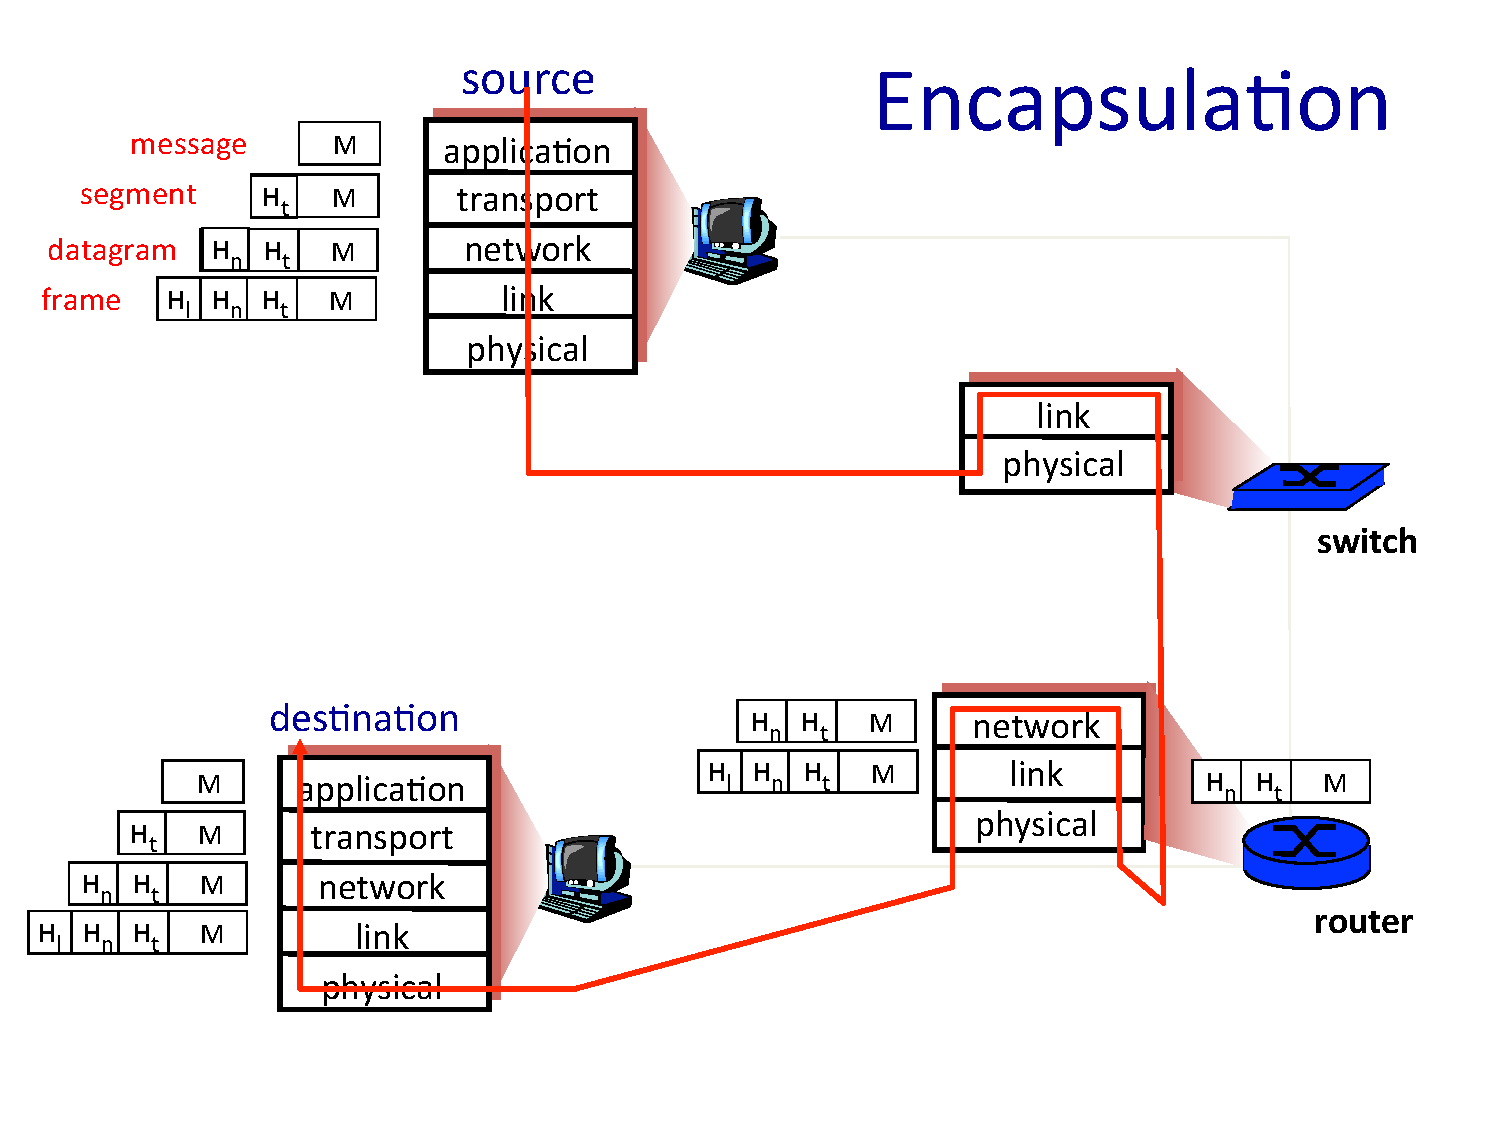
\includegraphics[width=\textwidth]{lazy/encapsulation.pdf}
\end{figure}